\begin{figure}[H]
\centering
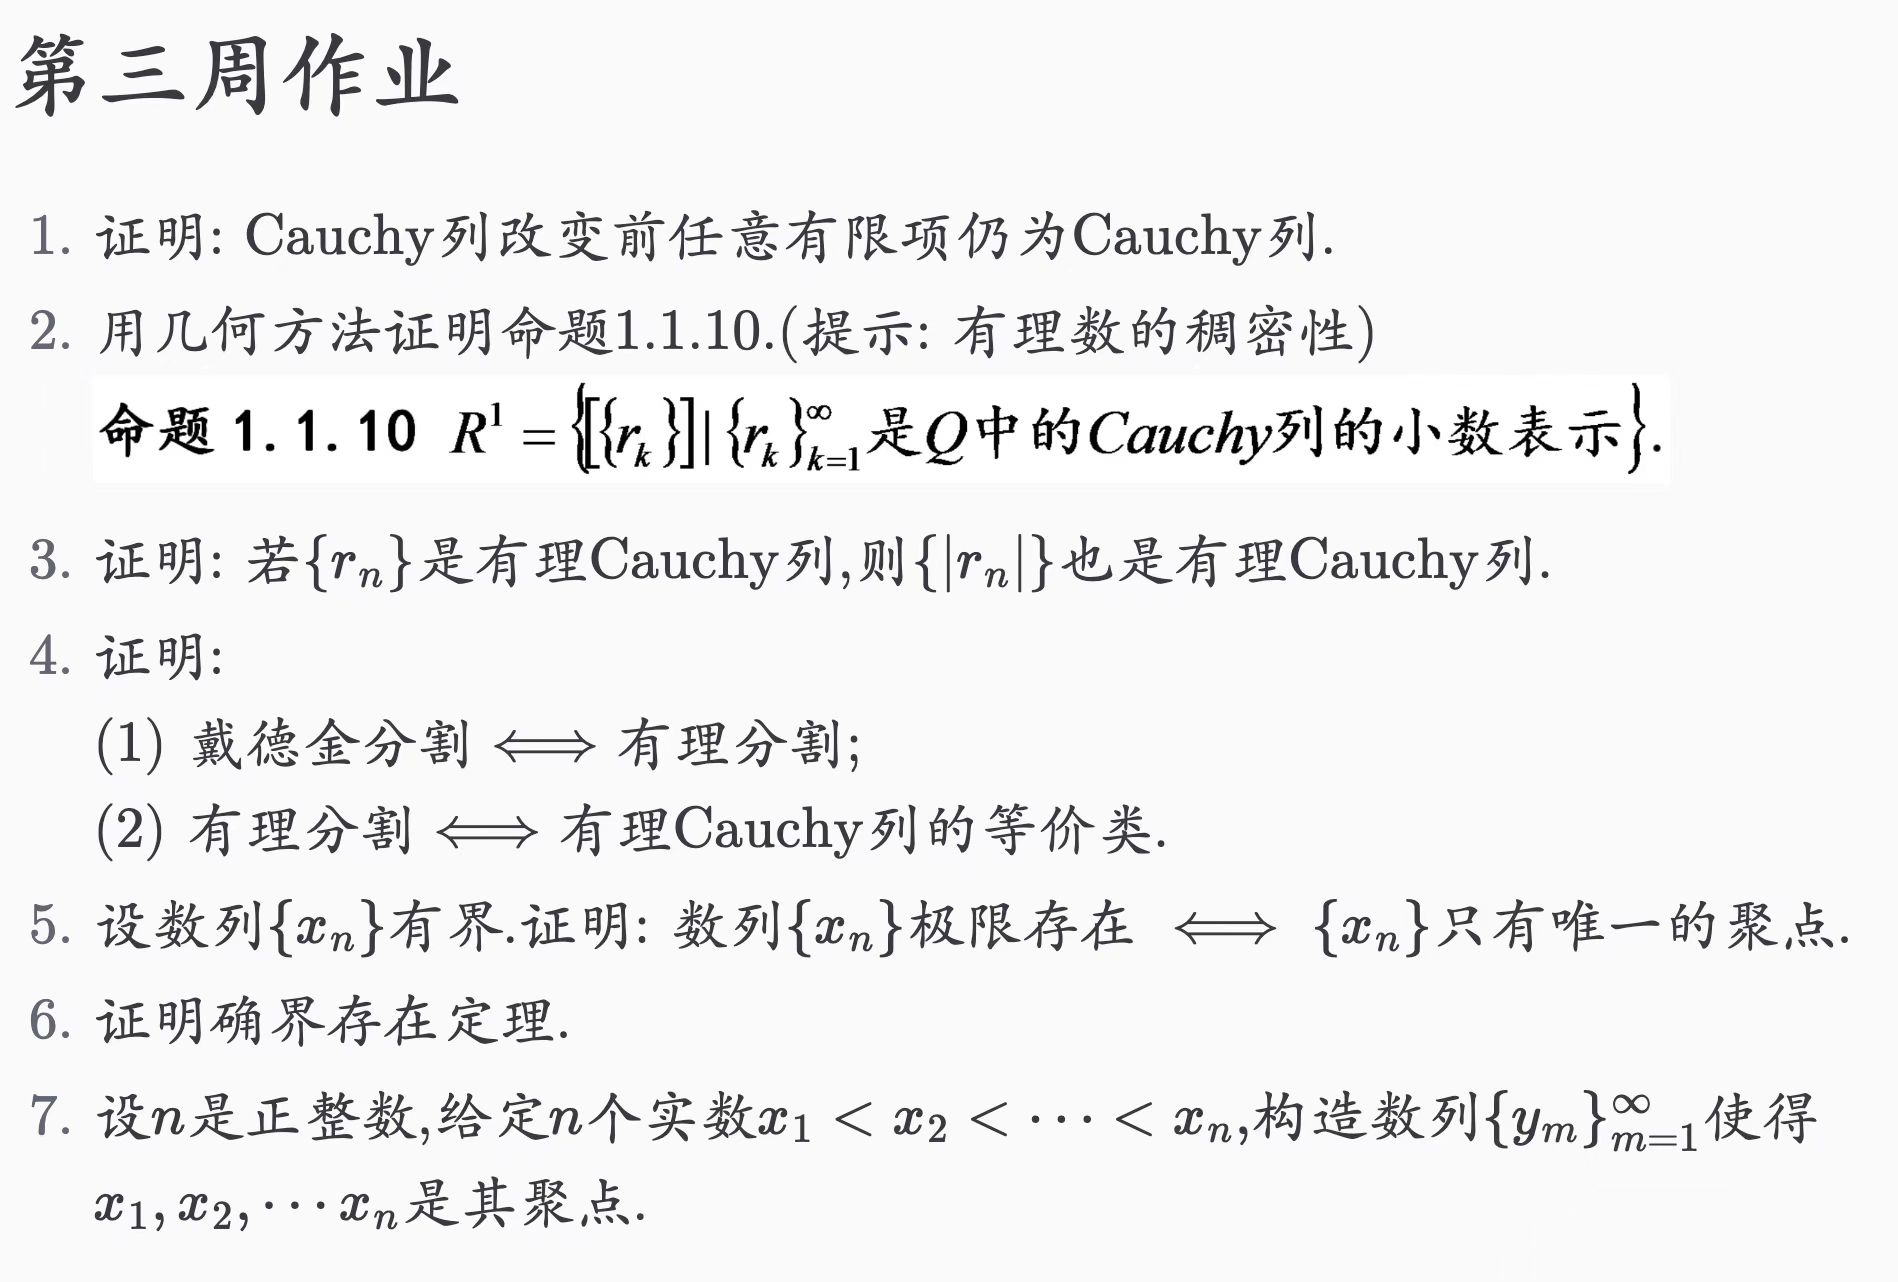
\includegraphics[width=\textwidth]{904841bf36031dff80d98b40c9fafc4.jpg}
% \caption{}
\label{}
\end{figure}

\begin{exercise}
证明:Cauchy 列改变前任意有限项仍为 Cauchy 列.
\end{exercise}
\begin{figure}[H]
\centering
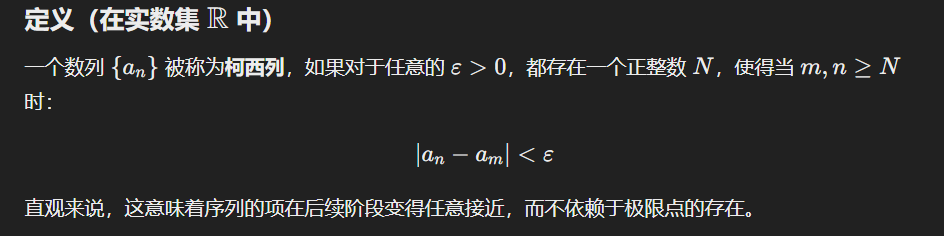
\includegraphics[width=\textwidth]{hw3-20250318.png}
% \caption{}
\label{}
\end{figure}

假设改变的有限项中指标最大的为 $a_{N'}$,那么对于任意的 $\varepsilon>0$,存在正整数 $\max\{ N,N' \}$ 是的当 $m,n\geq \max\{ N,N' \}$ 时,
\[
\lvert a_n-a_m \rvert <\varepsilon
\]
故得证 !

\begin{exercise}
用几何方法证明命题 1.1.10.(提示:有理数的稠密性)
\end{exercise}
\begin{proposition}
$R^1=\left\{\left[\left\{r_k\right\}\right] \mid\left\{r_k\right\}_{k=1}^{\infty}\right.$ 是 $Q$ 中的 Cauchy 列的小数表示 $\}$ .
\end{proposition}
显然!

\begin{exercise}
证明:若 $\left\{r_n\right\}$ 是有理 Cauchy 列,则 $\left\{\left|r_n\right|\right\}$ 也是有理 Cauchy 列.
\end{exercise}
\begin{figure}[H]
\centering
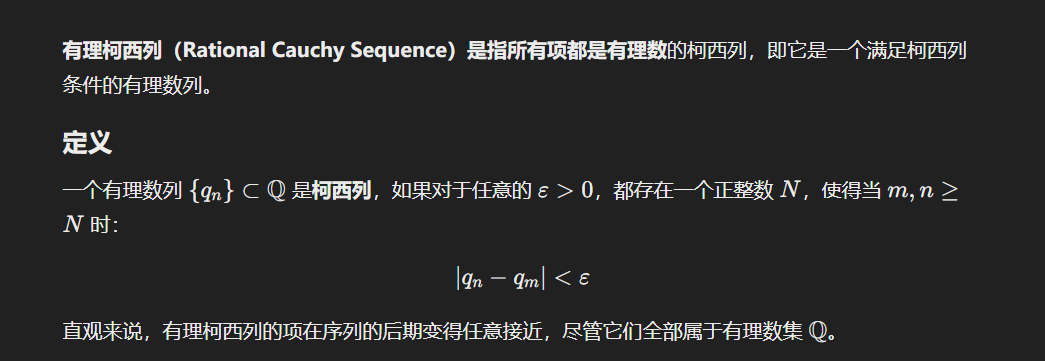
\includegraphics[width=\textwidth]{1-hw3-20250318.png}
% \caption{}
\label{}
\end{figure}

显然 $\lvert r_n \rvert\in \mathbb{Q},\forall n$. 由于 $\{ r_n \}$ 是有理 Cauchy 列,故对于任意 $\varepsilon>0$,存在 $N>0$,使得对于任意 $m,n>N$, 有
\[
\lvert r_m-r_n \rvert <\varepsilon
\]
于是
\[
\lvert \lvert r_m \rvert -\lvert r_n \rvert   \rvert \leq \lvert r_m-r_n \rvert<\varepsilon
\]
因此 $\{ \lvert r_n \rvert \}$ 也是有理 Cauchy 列.

\begin{exercise}
证明:
(1)戴德金分割 $\Longleftrightarrow$ 有理分割;
(2)有理分割 $\Longleftrightarrow$ 有理 Cauchy 列的等价类.
\end{exercise}
\begin{definition}[戴德金分割]
\begin{figure}[H]
\centering
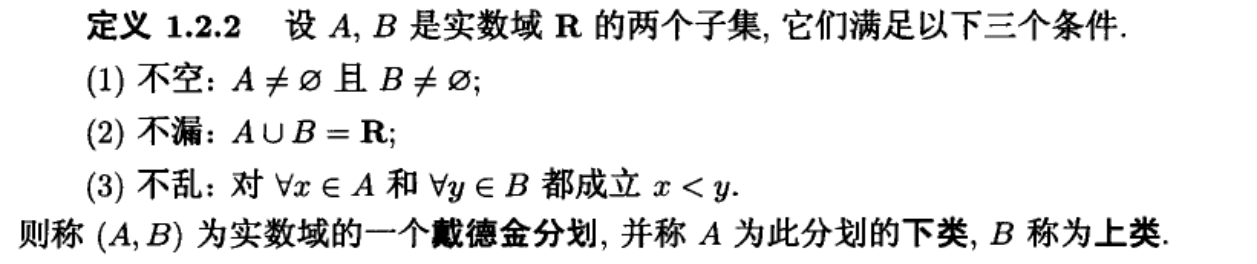
\includegraphics[width=\textwidth]{5-hw3-20250318.png}
% \caption{}
\label{}
\end{figure}
\end{definition}
\begin{definition}[有理分割]
\begin{figure}[H]
\centering

\includegraphics[width=\textwidth]{3-hw3-20250318.png}
% \caption{}
\label{}
\end{figure}
\end{definition}
戴德金分割 $\Rightarrow$ 有理分割: 根据戴德金原理,对于实数域的戴德金分割 $(A,B)$,要么下类 $A$ 中存在最大数,要么上类 $B$ 中存在最小数。无论如何,记这个数字为 $a$, 那么
\[
A=\{ r<a \},B=\{ r\geq a \}
\]
或者
\[
A=\{ r\leq a \},B=\{ r> a \}
\]
这是个有理分割。显然有理分割 $\Rightarrow$ 戴德金分割。故戴德金分割 $\Longleftrightarrow$ 有理分割

\begin{figure}[H]
\centering
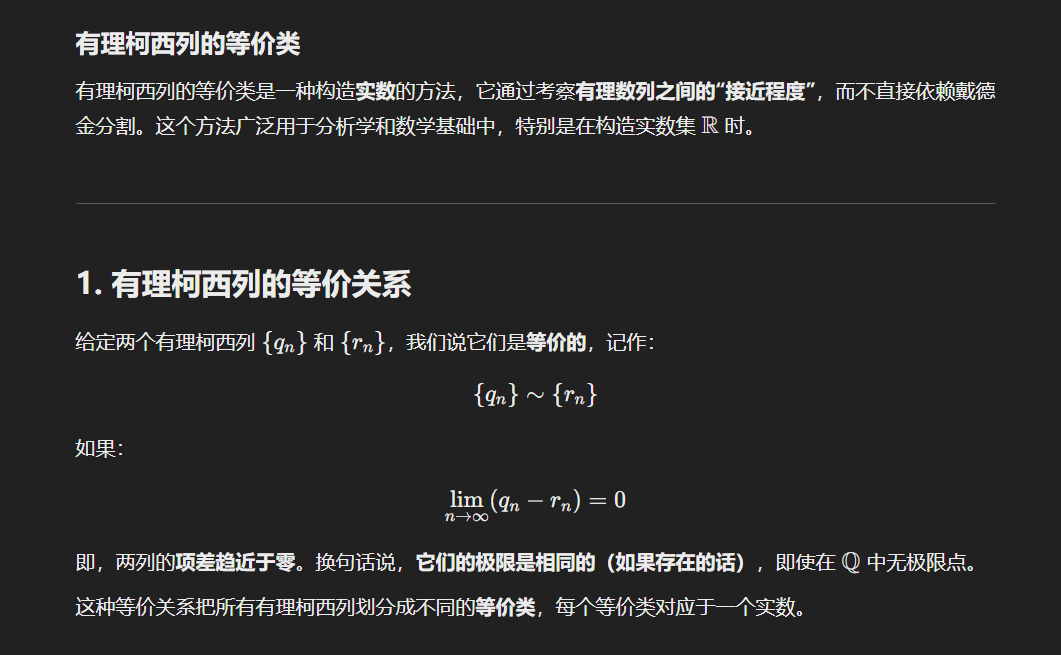
\includegraphics[width=\textwidth]{4-hw3-20250318.png}
% \caption{}
\label{}
\end{figure}

若 $(A,B)$ 是有理分割,分点为 $a\in \mathbb{Q}$,它对应等价类 $[a]$。若

\begin{exercise}
设数列 $\left\{x_n\right\}$ 有界.证明:数列 $\left\{x_n\right\}$ 极限存在 $\Longleftrightarrow\left\{x_n\right\}$ 只有唯一的聚点.
\end{exercise}
若 $x$ 是数列的极限,这等价于对于任意的 $\varepsilon>0$,存在 $N>0$,使得
\[
\lvert x_n-x \rvert <\varepsilon \qquad \forall n>N
\]
显然 $x$ 是 $\{ x_n \}$ 的聚点,假设 $y$ 也是聚点,那么存在 $N'>0$,使得
\[
\lvert x_n-y \rvert <\varepsilon \qquad \forall n>N'
\]
于是对于 $n>\max\{ N,N' \}$,有
\[
\lvert x-y \rvert \leq \lvert x-x_n \rvert +\lvert y-y_n \rvert <2\varepsilon
\]
由 $\varepsilon$ 任意性可知
\[
x=y
\]
只有唯一聚点。

另一个方向是显然的!

\begin{exercise}
证明确界存在定理.
\end{exercise}
根据戴德金定理:只要证明,若数集 $D$ 有上界,则 $D$ 必有唯一的上确界。
1.若 $D$ 有最大值 $M$ ,则 $M$ 就是 $D$ 的上确界。
2.设 $D$ 为无限集且无最大值。做实数集 $\mathbb{R}$ 的分割 $(X, Y)$ ,其中 $Y$ 为 $D$ 的一切上界所组成之集,$X$ 为 $Y$ 的补集。于是
(a)$X \neq \emptyset, Y \neq \emptyset$ .
(b)$X \cap Y=\emptyset$ ,
(c)任取 $x \in X$ ,若存在 $y \in Y$ 使 $y \leqslant x$ ,则 $x$ 成为 $D$ 的一个上界,从而 $x \in Y$ ,这与(b)矛盾。故对任意 $y \in Y, x \in X$ ,均有 $x<y$ 。

因此,$(X, Y)$ 是一个 Dedekind 分割。由分割原理,存在唯一 $\alpha \in \mathbb{R}$ ,使对任意 $x \in X, y \in Y$ 有
\[
x \leqslant \alpha<y \text { 或 } x<\alpha \leqslant y .
\]
因 $\alpha$ 不可能是 $X$ 的最大值(若 $\alpha$ 是 $X$ 的最大值,则 $\alpha \in Y$ ,从而 $X \cap Y \neq \emptyset$ .矛盾!)故对一切 $x \in X$ ,均有 $x<\alpha$ ,即 $x \leqslant \alpha<y$ 不能成立。这样,只有 $x<\alpha \leqslant y$ 成立,即 $\alpha$ 是 $Y$ 中的最小者,也就是 $D$ 的上界中的最小者,故 $D$ 有唯一的上确界 $\alpha$ 。

\begin{exercise}
设 $n$ 是正整数,给定 $n$ 个实数 $x_1<x_2<\cdots<x_n$ ,构造数列 $\left\{y_m\right\}_{m=1}^{\infty}$ 使得 $x_1, x_2, \cdots x_n$ 是其聚点.
\end{exercise}
我们可以构造数列 $\{ y^{(k)}_{m} \}_{m=1}^{\infty}\to x_k$,$k=1,2,\dots ,n$. 接下来令
\[
y_m=y^{(k)}_{r}\quad \text{if }m=n\cdot r+k
\]
其中 $1\leq k\leq n,r\geq0$. 于是 $x_1,x_2,\dots,x_n$ 是 $\{ y_m \}_{m=1}^{\infty}$ 的聚点.
